%%%%%%%%%%%%%%%%%%%%%%%%%%%%%%%%%%%%%%%%%%%%%%%%%%%%%%%%%%%%%%%%%%%%%%%%%%%%%%%%%%%%%%
%% Author:      Nils Weber and Maximilian Stiefel
%% Date:        23.12.2017
%% University:  Uppsala Universitet
%% Department:  Institutionen för informationsteknologi 
%% Course:      Embedded Control System Project
%% Project:     PRECISELY CONTROLLED DIY ETCHING MACHINE 
%%				FOR USAGE AT HOME AND IN SMALL LABS
%%%%%%%%%%%%%%%%%%%%%%%%%%%%%%%%%%%%%%%%%%%%%%%%%%%%%%%%%%%%%%%%%%%%%%%%%%%%%%%%%%%%%%

\chapter{Design}
\label{chap:design} 
\section{System Architecture and Required Functionality}
\label{sec:system_arch_and_req}
% Explain how our system is build up. 
First, the system consists out of two machines, the \gls{UV} light and the etching tank. Of course, these two machines are different and therefore need different designs. However, effort has been put into trying to use as many software and hardware components in both parts simultaneously to reduce the overall workload.  

\begin{figure}[H]                                                         
\centering          
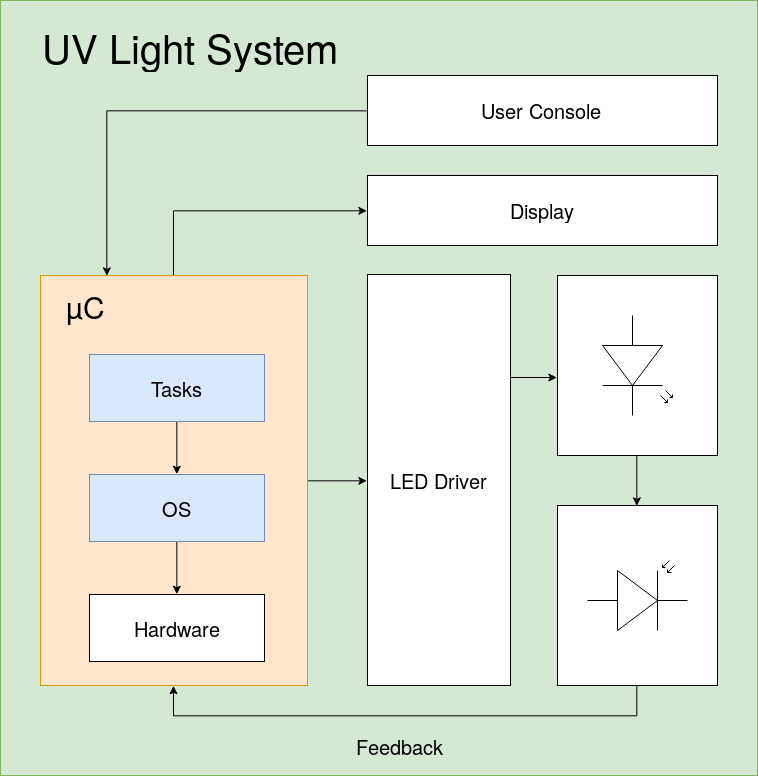
\includegraphics[width=0.5\textwidth]{./fig/uv_light_simple}   
\caption[\mu C with user interface, custom LED driver and feedback loop.]{\mu C on the left executing tasks with an OS below. User interface is hooked up to the \mu C. Custom LED driver is connected to LEDs, steered by software. Feedback comes from a light sensor.}   
\label{fig:uv_light_simple}
\end{figure}  

In fig. \ref{fig:uv_light_simple} a rough sketch of the \gls{UV} light exposure unit is shown. The most important part is probably the \glspl{LED} and the driver for it. A feedback from the \glspl{LED} is generated with the help of a light sensor. This feedback can be coupled into a controller steering the driver. Besides the \gls{LED} driver, one needs a microcontroller, that executes the \gls{OS} and tasks to implement the desired functionality. In addition, some components for communication with the user are necessary, i.e. a console and a display. The user must be able to adjust exposure time and intensity. The intensity is not changeable with devices currently available on the market. 

\begin{figure}[H]                                                         
\centering          
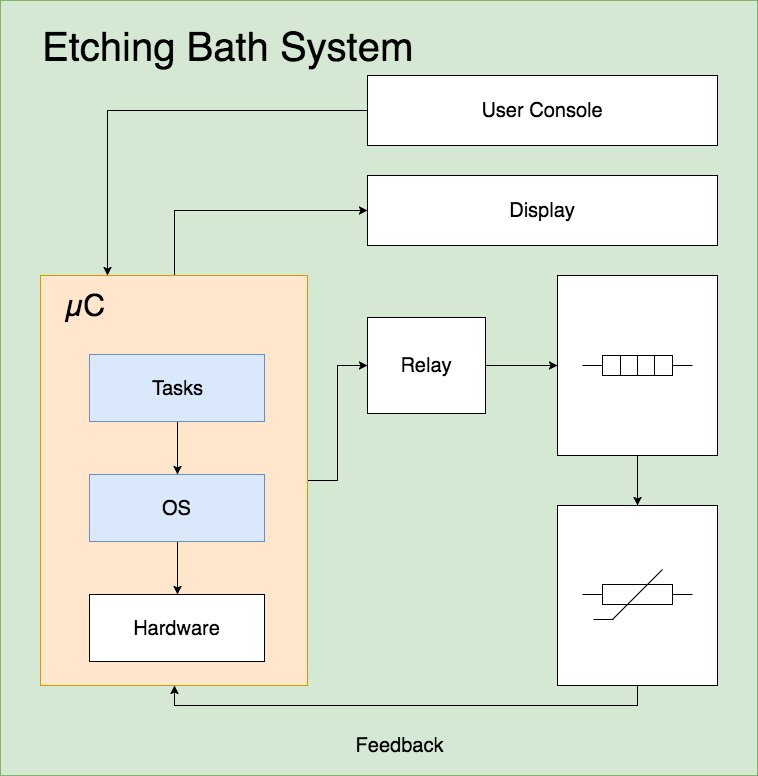
\includegraphics[width=0.5\textwidth]{./fig/etching_bath_simple}   
\caption[\mu C with user interface, heater and feedback loop.]{\mu C on the left executing tasks with an OS below. User interface is hooked up to the \mu C. The heater is connected via a relay, steered by software. Feedback comes from a temperature sensor.}   
\label{fig:etching_bath_simple}
\end{figure} 

In fig. \ref{fig:etching_bath_simple} the system architecture is sketched. Comparing to fig. \ref{fig:uv_light_simple} one can see many similarities, which result from the efforts to keep many parts of the system interchangable. The heater is not very sophisticated, thus the control is realized via a simple, optocoupled relay. An \gls{NTC} resistor is used as a temperature sensor and submersed into the etching bath. Thus, it closes the feedback loop for the control system.

Tab. \ref{tab:design_choices_uv_light} gives a bit more insights dealing with which components have been chosen and why. Also it includes information about the costs of each component. 

\section{Design Choices}
% Explain which design choices have been made and why.

The following table explains why different components have been chosen to enable the required functionality.

\begin{table}[H]
	\centering 
	\begin{tabular}{p{0.2\textwidth} p{0.2\textwidth} p{0.1\textwidth} 
		p{0.4\textwidth} } 
		\textbf{Block} &
		\textbf{Component(s)}&
		\textbf{Costs}& 
		\textbf{Justification of the
		Choice}\\\hline
		Microcontroller &
        STM32 microcontroller family &
        From 1.30 USD & 
        The µCs are cheap, because they are used everywhere. Open-source \glspl{IDE} are available and have a huge community. Open-source hardware is available as well. Big family tree with all kind of options. Powerful ARM Cortex-M0, Cortex-M3, Cortex-M4, Cortex-M7 32-bit processors. Ultra-low power (L-models) available. \\\hline 
        \gls{LED} Driver & 
        Custom designed linear regulator &
        0.40 USD per stage (25.60 USD for 64 stages) &
        One needs less components with a linear regulator (saves space and money). Choosing the voltage supply as close as possible to the voltage drop over the \gls{LED} or the \gls{LED} string, the efficiency is not too bad. Control part becomes very simple, yet effective. \\\hline
        Display &
        \gls{OLED} SSD1306 &
        2.50 USD &
        The display is cheap. Open-source driver software only needs to be ported to the platform. \gls{SPI} and \gls{I2C} interface available. \gls{OLED} technology is very elegant in comparison to alternatives.\\\hline
        User Console &
        Two rotary encoders and one tactile switch & 
        2 USD & 
        Very comfortable interface. One encoder for the exposure time, one for the light intensity and the tactile switch for starting the exposure process.\\
         &
        One rotary encoder including a push button & 
        \(<\) 1 USD & 
        Different parameters of the controller can be changed via the rotary encoder; the button is to switch between changing the parameter value or the parameter.\\\hline 
        Light Sensor &
        TSL2561 &
        1 USD & 
        Very easy to use with \gls{I2C} interface. Integrated amplifier. Very small. No need to develop a readout circuit with a photodiode.\\\hline 
        Temperature Sensor &
        NTCALUG01T103FL &
        3.5 USD & 
        Simple \gls{NTC} in metal package with ring connector. Robust, used in automotive applications. Comes with \SI{150}{\milli\metre} of wire. Detailed support from manufacturer.\\\hline
        Relay with optocoupler &
        - &
        \(<\) 1 USD & 
        Simple and safe to use via digital out.\\\hline 
        Air Temperature Sensor &
        SHT31 &
        4 USD & 
        Highly accurate air temperature and humidity sensor. Includes \gls{I2C}-interface.\\\hline
	\end{tabular}
	\caption{Design choices for the system: Why has each component been chosen?}
	\label{tab:design_choices_uv_light}
\end{table}




\section{Mathematical Model of the Tank}

Using the concept of energy balance to describe the thermodynamical model of the tank yields following equations \cite{online:mathModel}:
\begin{equation*}
Heat_{in} = Heat_{out} + Heat_{stored}
\end{equation*}

\begin{equation}
q_i=\frac{\theta_t - \theta_e}{R_{ta}}+c\frac{d\theta_t}{dt}
\end{equation}

with \(c\) as heat capacity of water, 4184\si{\frac{\joule}{\kilogram\kelvin}}, and
\(R_{ta}\) as temperature resistance between tank and ambient environment.

To further develop a model, different measurements are necessary. Water has a different specific heat capacity in different phases, i.e. as ice or water \cite{online:watercurve}.
\begin{equation}
q=m*C_s*\Delta T
\end{equation}

Different measurements to gather data to further build and understand the mathematical system. All measurements are to be done with the original water tank, heater and the temperature sensor.
\begin{itemize}
\item Cooling behavior 
	\begin{itemize}
	\item Measure temperature every 10s while cooling down water 
	\item Start from different temperatures
	\end{itemize}
\item Heating behavior
	\begin{itemize}
	\item Measure temperature every 10s while heating up water
	\end{itemize}
\item Determine time constants
\end{itemize}





